%\documentclass[12pt]{article}
%\usepackage[a4paper, margin=1in]{geometry} 
%\usepackage{graphicx} 
%\usepackage{hyperref}
%\usepackage{float}
%\usepackage{multicol}
%\usepackage{multirow}
%\usepackage[font=small, labelfont=bf]{caption}
%\usepackage[table,xcdraw]{xcolor}
%
%\begin{document}

%
% Evaluation of local alignment
%
\subsection{Evaluation of local alignment}
The underlying distribution of local alignment scores is an extreme value distribution.

%
% Gumbel distribution
%
\subsubsection*{Gumbel distribution} 
The Gumbel distribution is a member of the extreme value distribution family. \\

\begin{figure}[H]
  \centering
      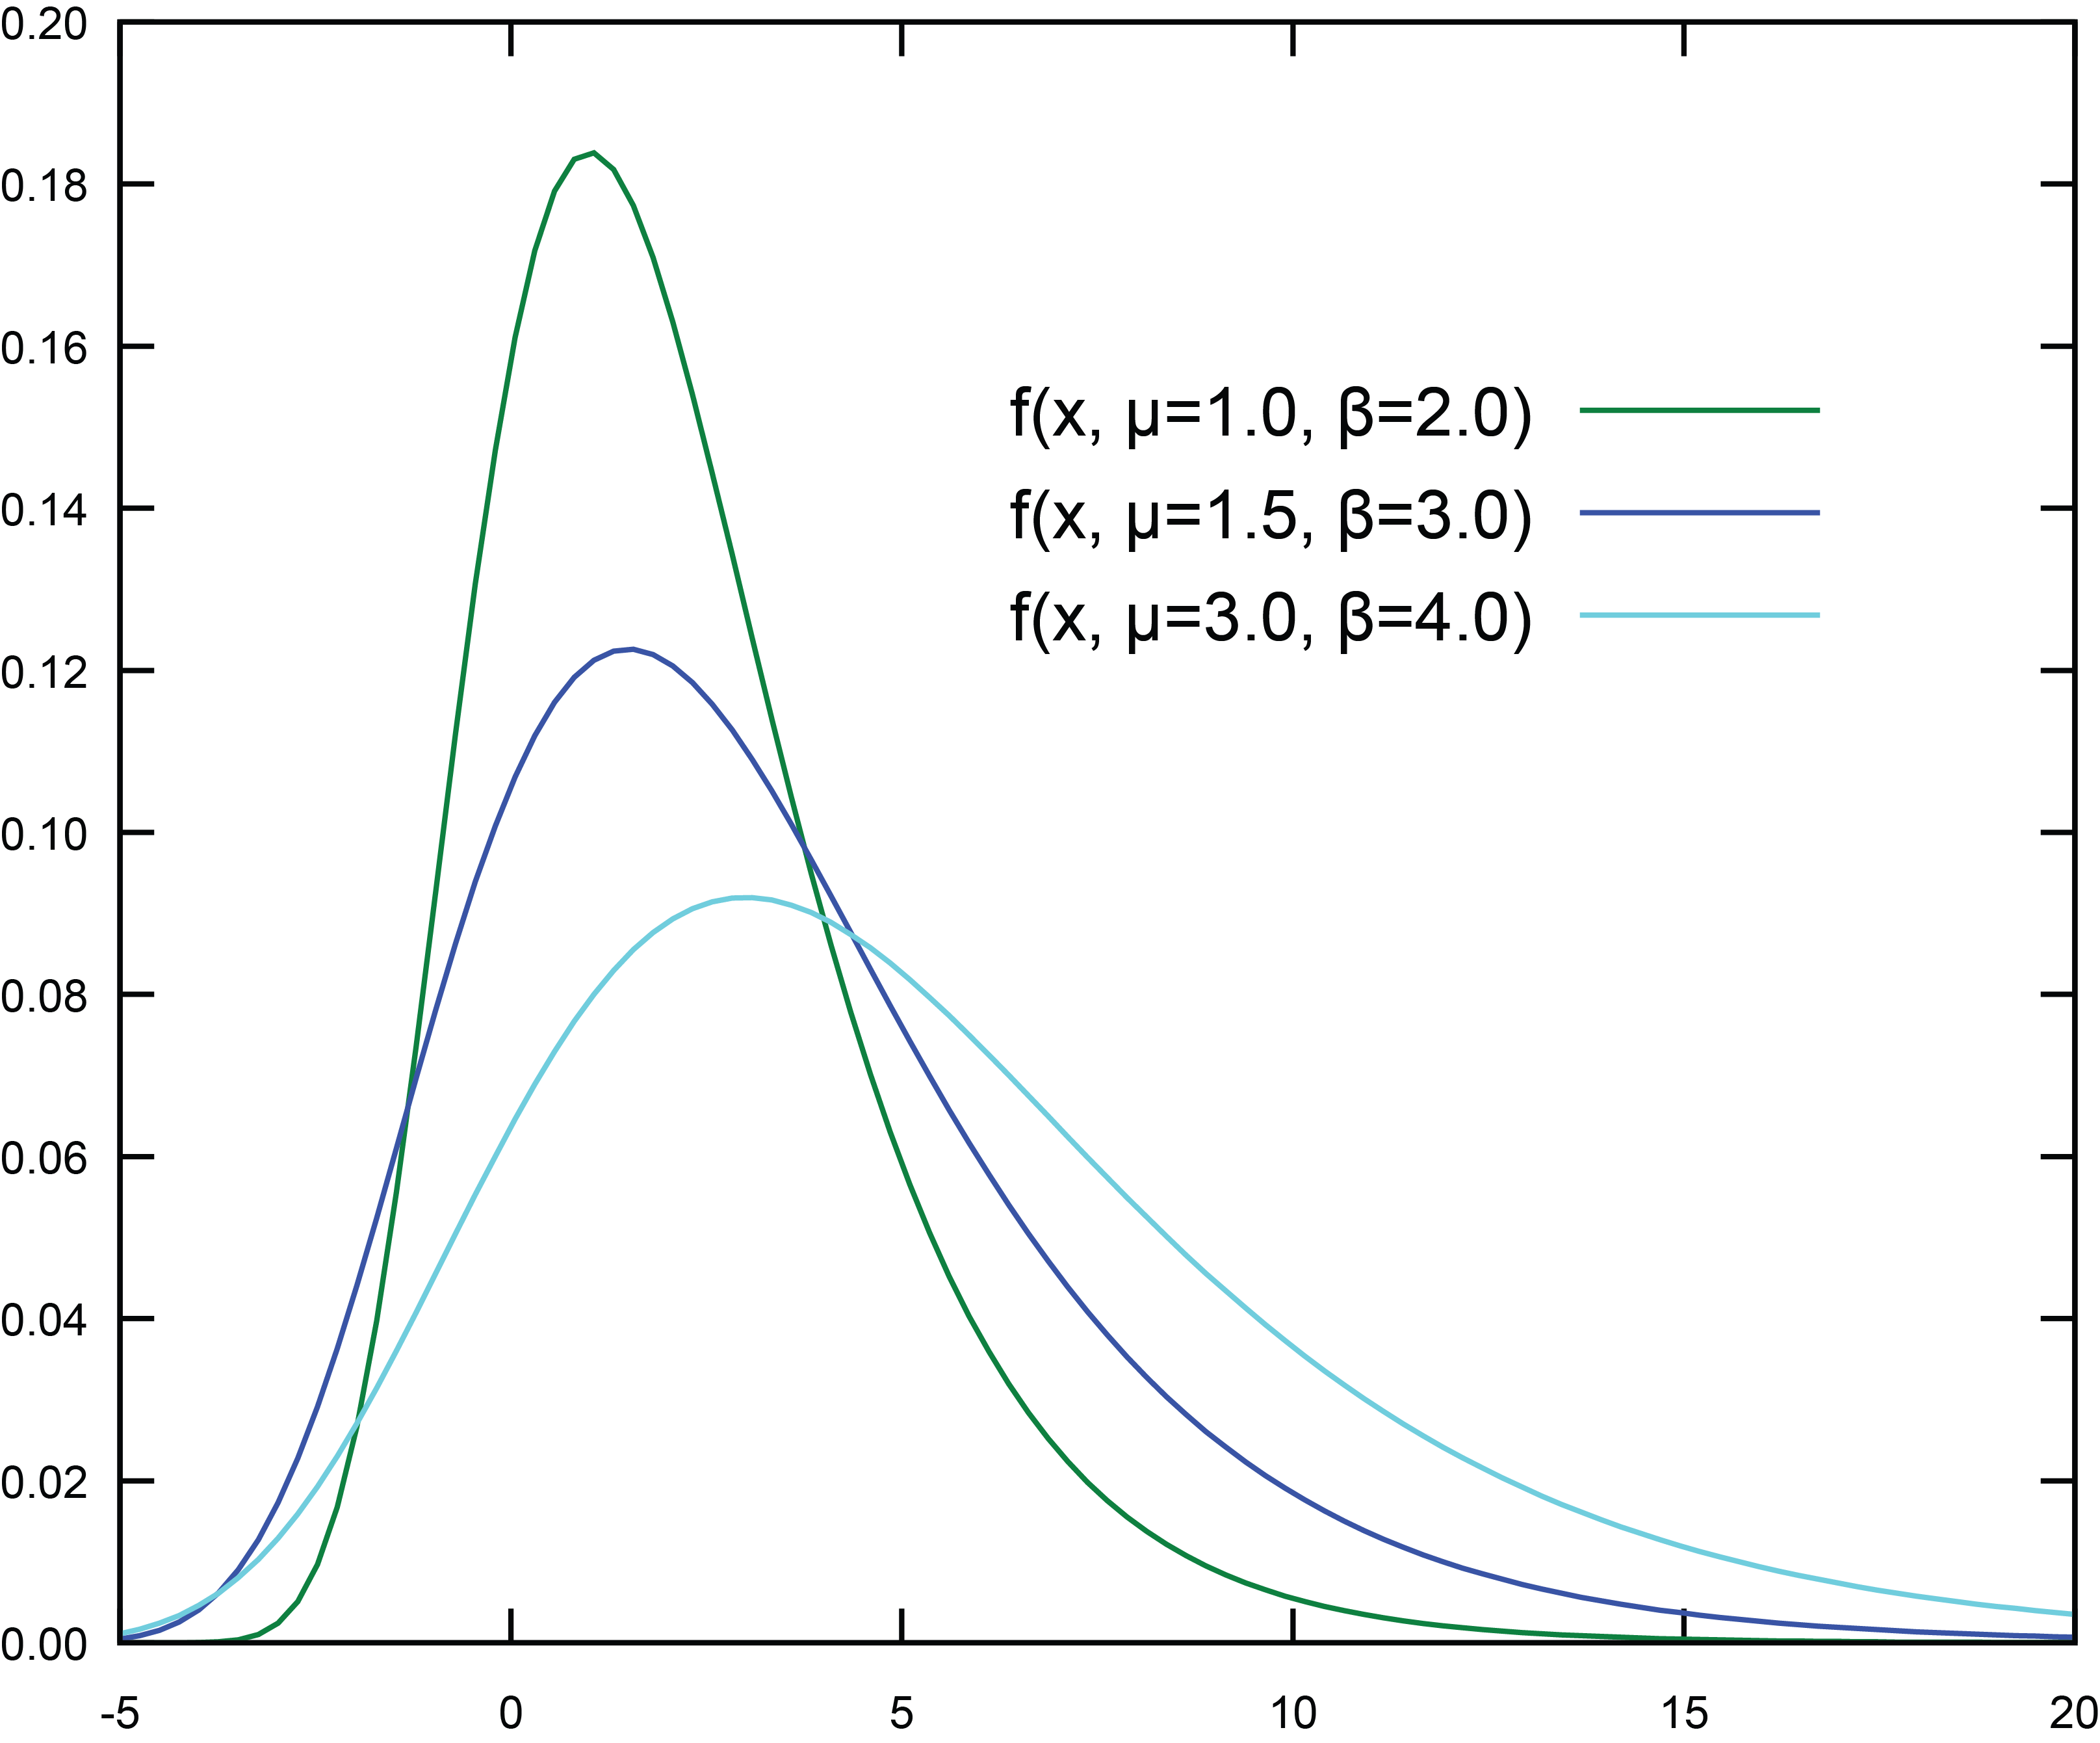
\includegraphics[width=0.4 \textwidth]{fig06/gumbel.png}
  \caption{Gumbel distribution (source: \href{https://commons.wikimedia.org/w/index.php?curid=4787663}{Herr blaschke, Wikimedia Commons})}
\end{figure}

\noindent
The cumulative distribution function (CDF) of the Gumbel distribution: \\

$F_Y(y) = exp⁡[-e^{-\lambda(y-\mu)}]$ \\

\noindent
Parameters
\begin{itemize}
\item $\mu$: the modal value of the distribution, characteristic value
\item $\lambda$: a measure of the variance, decay constant
\end{itemize}

%
% Extreme value distribution
%
\subsubsection*{Extreme value distribution}
An extreme value distribution is a limiting distribution for the minimum or the maximum of a sufficiently large sample. Ungapped alignments with large sequence lengths are known to have this type of distribution. \\

\noindent
\textbf{Example (m and n are not large in this example)}

\begin{table}[H]
\centering
\begin{tabular}{lllllllll}
                       &                        & A                        & C                                                & G                                              & C                        & A                        & C                                                & G                                              \\ \cline{2-9} 
\multicolumn{1}{l|}{}  & \multicolumn{1}{l|}{0} & \multicolumn{1}{l|}{0}   & \multicolumn{1}{l|}{0}                           & \multicolumn{1}{l|}{0}                         & \multicolumn{1}{l|}{0}   & \multicolumn{1}{l|}{0}   & \multicolumn{1}{l|}{0}                           & \multicolumn{1}{l|}{0}                         \\ \cline{2-9} 
\multicolumn{1}{l|}{C} & \multicolumn{1}{l|}{0} & \multicolumn{1}{l|}{0}   & \multicolumn{1}{l|}{\cellcolor[HTML]{FE0000}0.5} & \multicolumn{1}{l|}{0}                         & \multicolumn{1}{l|}{0.5} & \multicolumn{1}{l|}{0}   & \multicolumn{1}{l|}{\cellcolor[HTML]{FE0000}0.5} & \multicolumn{1}{l|}{0}                         \\ \cline{2-9} 
\multicolumn{1}{l|}{G} & \multicolumn{1}{l|}{0} & \multicolumn{1}{l|}{0}   & \multicolumn{1}{l|}{0}                           & \multicolumn{1}{l|}{\cellcolor[HTML]{FE0000}1} & \multicolumn{1}{l|}{0.5} & \multicolumn{1}{l|}{0.2} & \multicolumn{1}{l|}{0}                           & \multicolumn{1}{l|}{\cellcolor[HTML]{FE0000}1} \\ \cline{2-9} 
\multicolumn{1}{l|}{A} & \multicolumn{1}{l|}{0} & \multicolumn{1}{l|}{0.5} & \multicolumn{1}{l|}{0}                           & \multicolumn{1}{l|}{0.5}                       & \multicolumn{1}{l|}{0.7} & \multicolumn{1}{l|}{0.2} & \multicolumn{1}{l|}{0}                           & \multicolumn{1}{l|}{0.5}                       \\ \cline{2-9} 
\end{tabular}
\end{table}

\begin{table}[H]
\centering
\begin{tabular}{
>{\columncolor[HTML]{FE0000}}l |
>{\columncolor[HTML]{FE0000}}l |l|l|l|l|l}
CG & CG & GC  &     & AC   &     &     \\
CG & CG & GA  & ... & CG   & ... & ... \\ \hline
1  & 1  & 0.2 &     & -0.6 &     &    
\end{tabular}
\end{table}

%
% Parameter estimation
%
\subsubsection*{Parameter estimation}
The p-value of the Gumbel distribution can be calculated as: \\

$P[Y>y]=1-F_Y (y)=1-exp⁡[-e^{-\lambda(y-\mu)}]$ \\

\noindent
The parameters $\mu$ and $\lambda$ can be estimated from the arithmetic mean $m_{Y}$ and the variance $\sigma_{Y}^2$ of the observed sample. \\

$\lambda \approx 1.282 / \sigma_{Y}$ \\

$\mu \approx m_{Y} - 0.577/\lambda$

%
% Example of parameter estimation
%
\subsubsection*{Example of parameter estimation}
Below is the optimal local alignment with the score between q:ACAGACTACTA and  d:TCAGACTGGGAACCE.

\begin{verbatim}
    CAGACT
    CAGACT
    Score: 6
\end{verbatim}

\noindent
The mean and the variance of the alignment scores are estimated as follows from randomly generated sequences. \\

$m_{Y}$: 1.7221 \\

$\sigma_{Y}$: 1.6025 \\

\noindent
Then, $\lambda$ and $\mu$ are estimated from $m_{Y}$ and $\sigma_{Y}$. \\

$\lambda \approx 1.282 / 1.6025 = 0.8$ \\

$\mu \approx 1.7221- 0.577/0.8 \approx 1$  \\

\noindent
The p-value is approximately 0.0181 when $\lambda = 0.8$ and $\mu = 1$ . The test result is statistically significant ($\alpha$= 0.05), and therefore, the null hypothesis is rejected. \\

\noindent
\textbf{Conclusion:} The query and the database sequences are homologous (p-value: 0.0181).

\bigskip 

%\end{document}
